\documentclass[hyperref={pdfpagelabels=false},table,10pt,compress]{beamer}


%%%%%%%%%%%%%%%%%%%%%%%%%%%%%% BEGIN-Packages %%%%%%%%%%%%%%%%%%%%%%%%%%%%%
\usepackage{amsmath,amssymb,amsfonts}
\usepackage{mathrsfs,enumerate}
\usepackage{color,xcolor}
\usepackage{graphicx,subfigure}
\usepackage{clock} % Use this package to insert a clock in the beamer.
\usepackage{textcomp}
\usepackage[T1]{fontenc}
\usepackage{verbatim}
\usepackage{moreverb}
\usepackage{booktabs}
\usepackage{tabularx}
\usepackage{multirow,multicol}
\usepackage{natbib}
\usepackage[ruled,lined,linesnumbered]{algorithm2e}
%\usepackage{algorithm2e}
%\usepackage{url}
%\usepackage{hyperref}
\usepackage[colorlinks,linkcolor=black,citecolor=black,urlcolor=black]{hyperref}%[colorlinks,linkcolor=blue,citecolor=blue,urlcolor=blue]
\usepackage{CJK}
%%%%%%%%%%%%%%%%%%%%%%%%%%%%%%%% END-Packages %%%%%%%%%%%%%%%%%%%%%%%%%%%%%


% \setbeamertemplate{navigation symbols}{} % Disable the buttons at the bottom.

\graphicspath{{Figures/}} % Set the directory where figures are saved.

%%%%%%%%%%%%%%%%%%%% BEGIN-Theorem-like Environments %%%%%%%%%%%%%%%%%%%%%
%\newtheorem{mybox}{}
\newtheorem{Con}{Conjecture}[section]
\newtheorem{Thm}{Theorem}[section]
\newtheorem{Prop}{Proposition}[Thm]
%%%%%%%%%%%%%%%%%%%%% END-Theorem-like Environments %%%%%%%%%%%%%%%%%%%%%%


%%%%%%%%%%%%%%%%%%%%%%%%%% BEGIN-New Commands %%%%%%%%%%%%%%%%%%%%%%%%%%%%
\newcommand{\email}[1]{\href{mailto: #1}{\tt {\color{blue}#1}}}
\newcommand{\red}{\color{red}}
\newcommand{\blue}{\color{blue}}
\newcommand{\green}{\color{green}}
\newcommand{\brown}{\color{brown}}
\newcommand{\orange}{\color{orange}}
\newcommand{\yellow}{\color{yellow}}
\newcommand{\white}{\color{white}}
\newcommand{\Real}{\mathbb{R}}
\newcommand{\Tran}[1]{#1^\mathrm{T}}
\newcommand{\st}{\textnormal{s.t.}}
\newcommand{\dist}{\textnormal{dist}}
\newcommand{\bc}{\begin{center}}
\newcommand{\ec}{\end{center}}
\newcommand{\bl}{\begin{flushleft}}
\newcommand{\el}{\end{flushleft}}
\newcommand{\tbf}{\textbf}
\newcommand{\be}{\begin{equation}}
\newcommand{\ee}{\end{equation}}
\newcommand{\ba}{\begin{array}}
\newcommand{\ea}{\end{array}}
\newcommand{\btab}{\begin{table}\begin{tabular}}
\newcommand{\etab}{\end{tabular}\end{table}}
\newcommand{\nn}{\nonumber}
\newcommand{\xn}{x_1,x_2,\ldots,x_n}
\newcommand{\framee}[2]{\frame{\frametitle{#1} #2}}
\newcommand{\reff}[1]{(\ref{#1})} % 免得敲()
\newcommand{\inner}[2]{\left\langle#1,#2\right\rangle}
\newcommand{\paper}[1]{({\blue \footnotesize{#1}})}
\newcommand{\hd}[1]{\multicolumn{1}{c}{#1}}


\newcommand{\rmnum}[1]{\romannumeral #1}
\newcommand{\Rmnum}[1]{\expandafter\@slowromancap\romannumeral #1@}
%%%%%%%%%%%%%%%%%%%%%%%%%%%% END-New Commands %%%%%%%%%%%%%%%%%%%%%%%%%%%%

\usepackage[ruled]{algorithm2e}

\begin{document}
\begin{CJK*}{GBK}{kai}

\title[distance geometry]{\textsc{A Buildup-based Error Minimization Method with Application to Protein Structure Determination}}
\author[Zhenli Sheng]{Zhenli Sheng (ʢ����)\\email: {\blue szl@lsec.cc.ac.cn}}
% \institute{Institute of Computational Mathematics and Scientific/Engineering Computing}
\institute[ICMSEC, CAS]{Institute of Computational Mathematics and Scientific/Engineering Computing,\\Chinese Academy of Sciences}
\date[]{April 9th, 2013\\ seminar talk}
\frame{
\titlepage
}

% File Name: ThankYou.tex
% Function: Insert an Outline page.


\section*{\textsc{Outline}}
\begin{frame}
\frametitle{\textsc{Outline}}
\end{frame}

\begin{frame}
\frametitle{\textsc{Outline}}
\tableofcontents[pausesections]
\end{frame}

\section{Problem Introduction}
\frame{
\frametitle{the Problem}
%\begin{block}{Molecular Conformation (Protein Structure Determination)}
%Given some interatomic distances, realize the structure of the protein.
%\end{block}

\begin{block}{Distance Geometry Problem (DGP)}
For a graph $G=(V,E)$, given a distance matrix $D$ ($L$ and $U$, respectively) on $E$ and an integer $d$, find $x_1,x_2,\ldots,x_n \in \Real^d$, such that
\begin{displaymath}
\|x_{i}-x_{j}\|=d_{ij},\quad (i,j) \in E.
\end{displaymath}
or
$$l_{ij}\leq \|x_i-x_j\|\leq u_{ij},\quad (i,j) \in E.$$
\end{block}
}

\framee{Related Applications/Problems}{
Some closely related applications/problems:
\begin{itemize}
  \item Sensor network localization
    \begin{itemize}
        \item $d=2$, anchors
    \end{itemize}
  \item Protein structure determination (molecular conformation)
    \begin{itemize}
        \item $d=3$, no anchors
    \end{itemize}
  \item Graph realization
  \item Dimensionality reduction
    \begin{itemize}
      \item $d$ unknown, "distances" need be constructed
    \end{itemize}
  \item Euclidean matrix completion
\end{itemize}
\vskip3mm
Note that
\begin{itemize}
  \item In most cases, the distances are {\blue local} and {\blue sparse}.
  \item Usually, the distances are {\blue noisy}.
\end{itemize}
}

\framee{}{
\begin{figure}
  \centering
  \subfigure{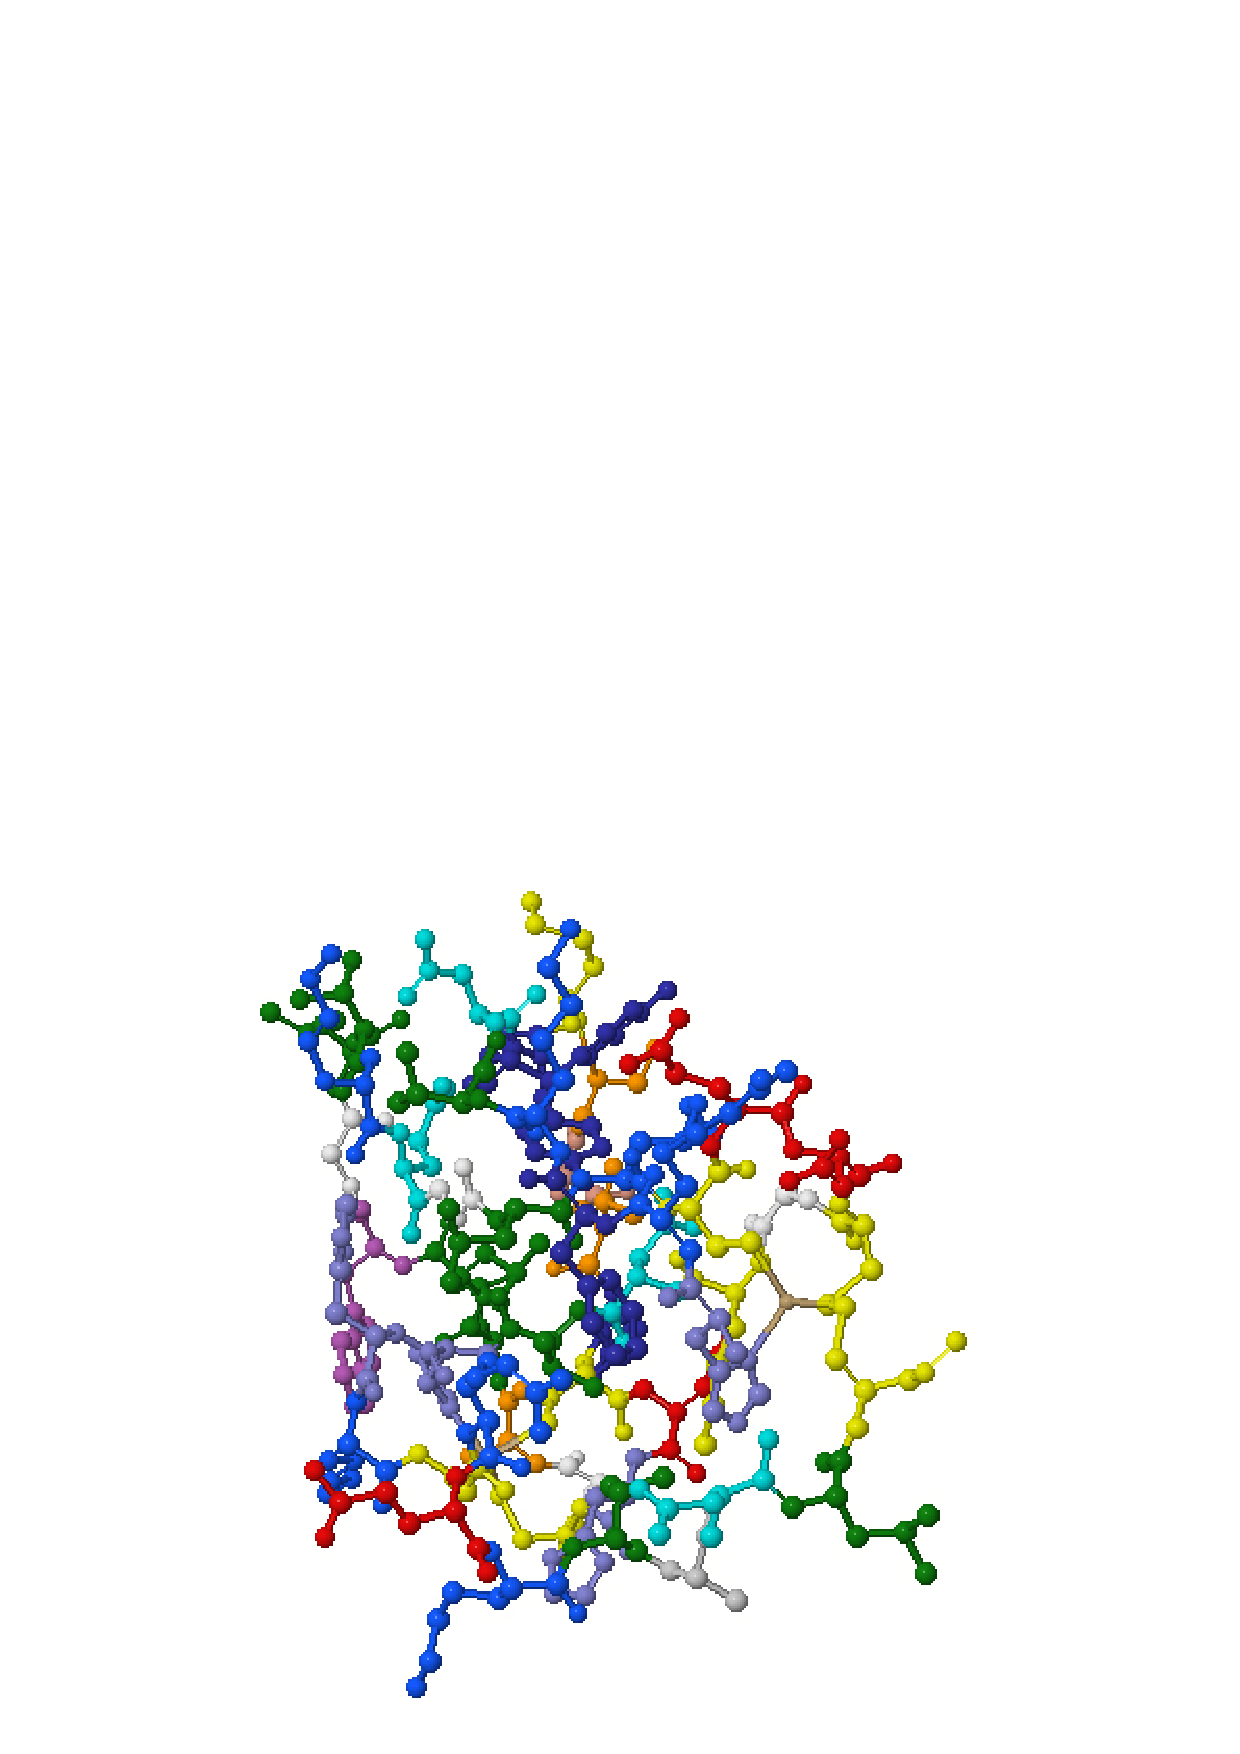
\includegraphics[width=0.45\textwidth]{1PTQ.jpg}}
  \subfigure{\includegraphics[width=0.45\textwidth]{1HQQ.jpg}}
  \subfigure{\includegraphics[width=0.45\textwidth]{sensor2.jpg}}
  \subfigure{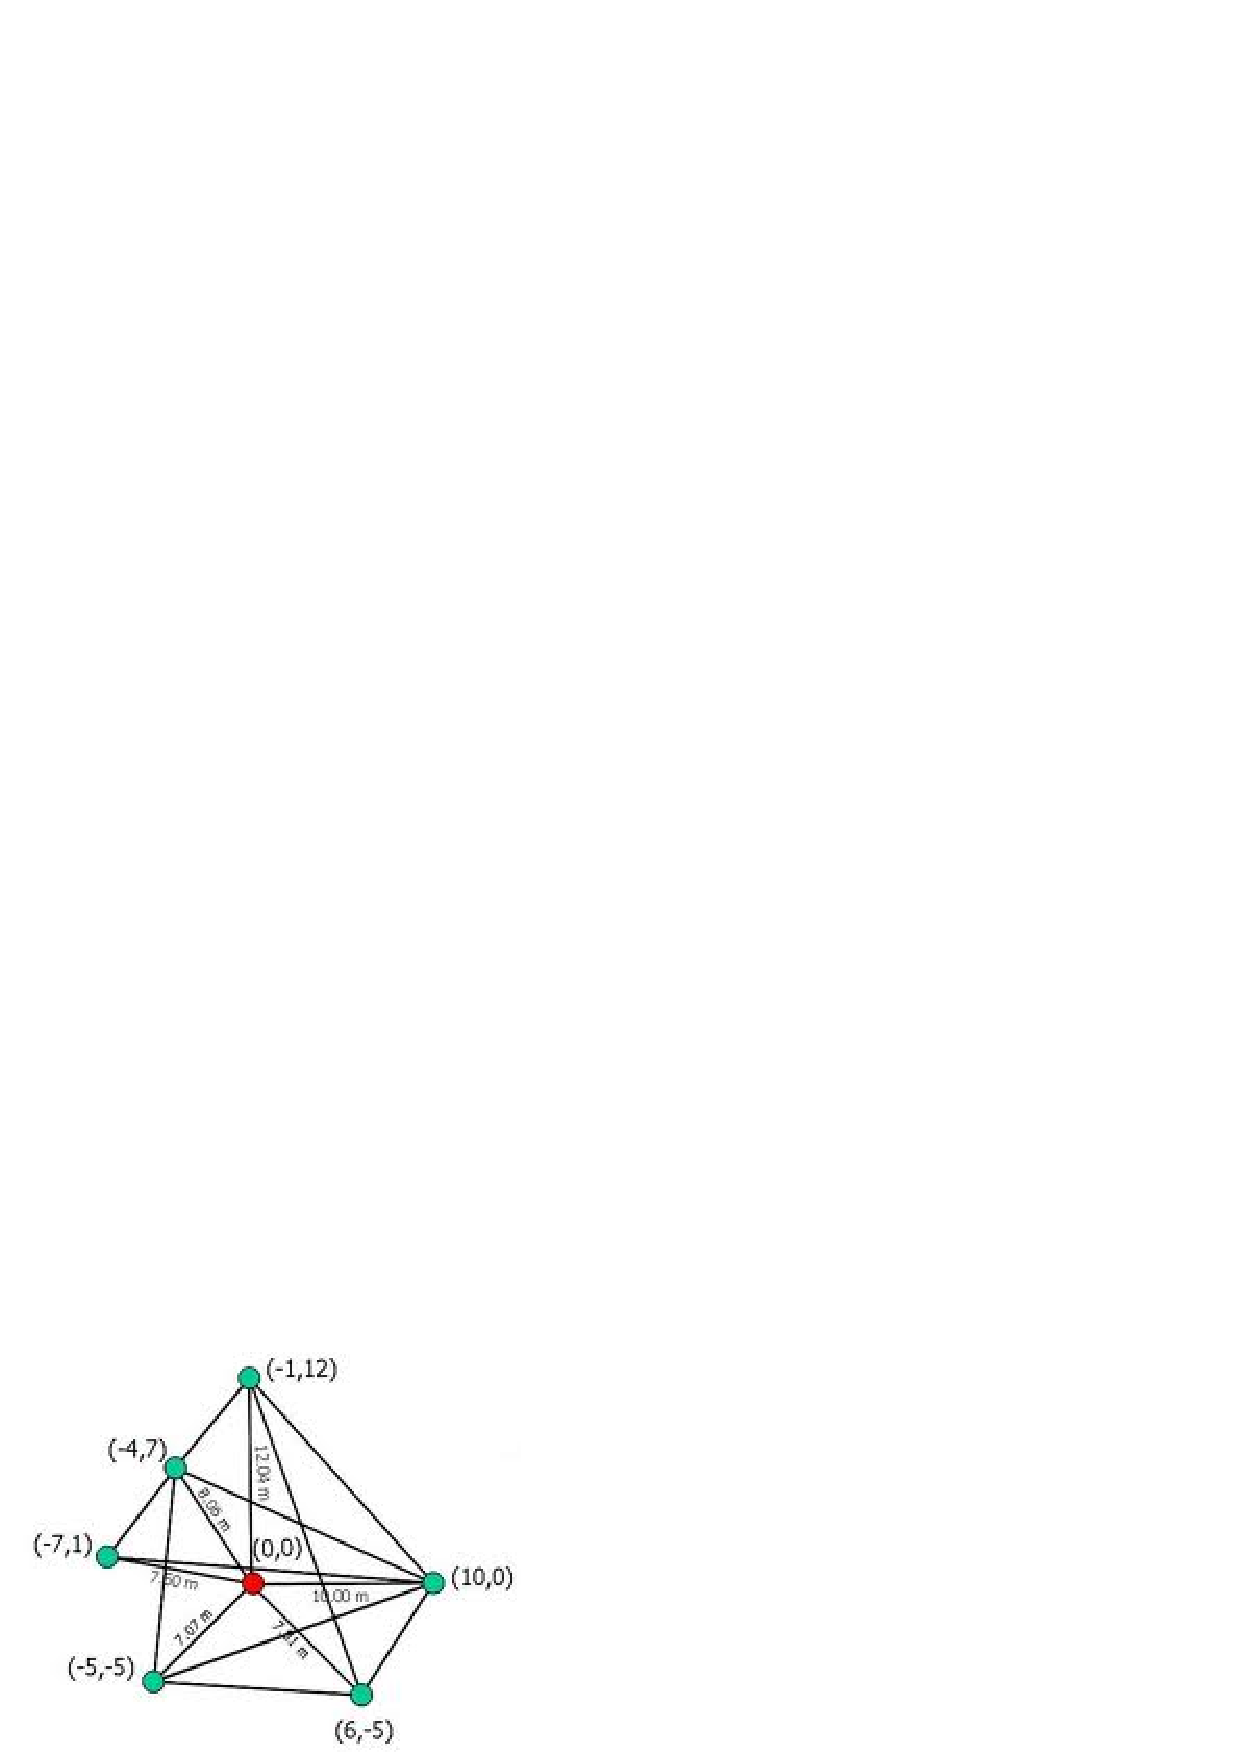
\includegraphics[width=0.45\textwidth]{GraphRealization.jpg}}
\end{figure}
}

\framee{Solution Methods}{
\begin{itemize}
  \item Matrix Decomposition Method \paper{Blumenthal 1953, Torgerson,1958}
  \item The Embedding Algorithm \paper{Crippen-Havel, 1988}
  \item Global Smoothing Algorithm \paper{Mor$\acute{e}$-Wu, 1997}
  \item Geometric Buildup Method \paper{Dong-Wu, 2002, Sit-Wu-Yuan, 2009}
  \item SDP Relaxation Method \paper{Biswas-Toh-Ye, 2007}
  \item Nearest Euclidean Distance Matrix \paper{Qi-Yuan, 2013}
  \item The Branch-and-Prune Algorithm \paper{Liberti-Lavor-Maculan-Mucherino, 2014}
\end{itemize}

\vskip3mm
Remark that
\begin{itemize}
  \item Those are just some representative papers.
  \item Rigidity is also a very important problem.
\end{itemize}
}

%\section{Maximal Variance Unfolding (MVU) Regularization}

\section{Laplacian Eigenmap-based Algorithm}
\subsection{Laplacian Eigenmap}

\framee{Motivation}{
\begin{figure}
  \centering
  \subfigure{\includegraphics[width=0.45\textwidth]{eigenone.png}}
  \subfigure{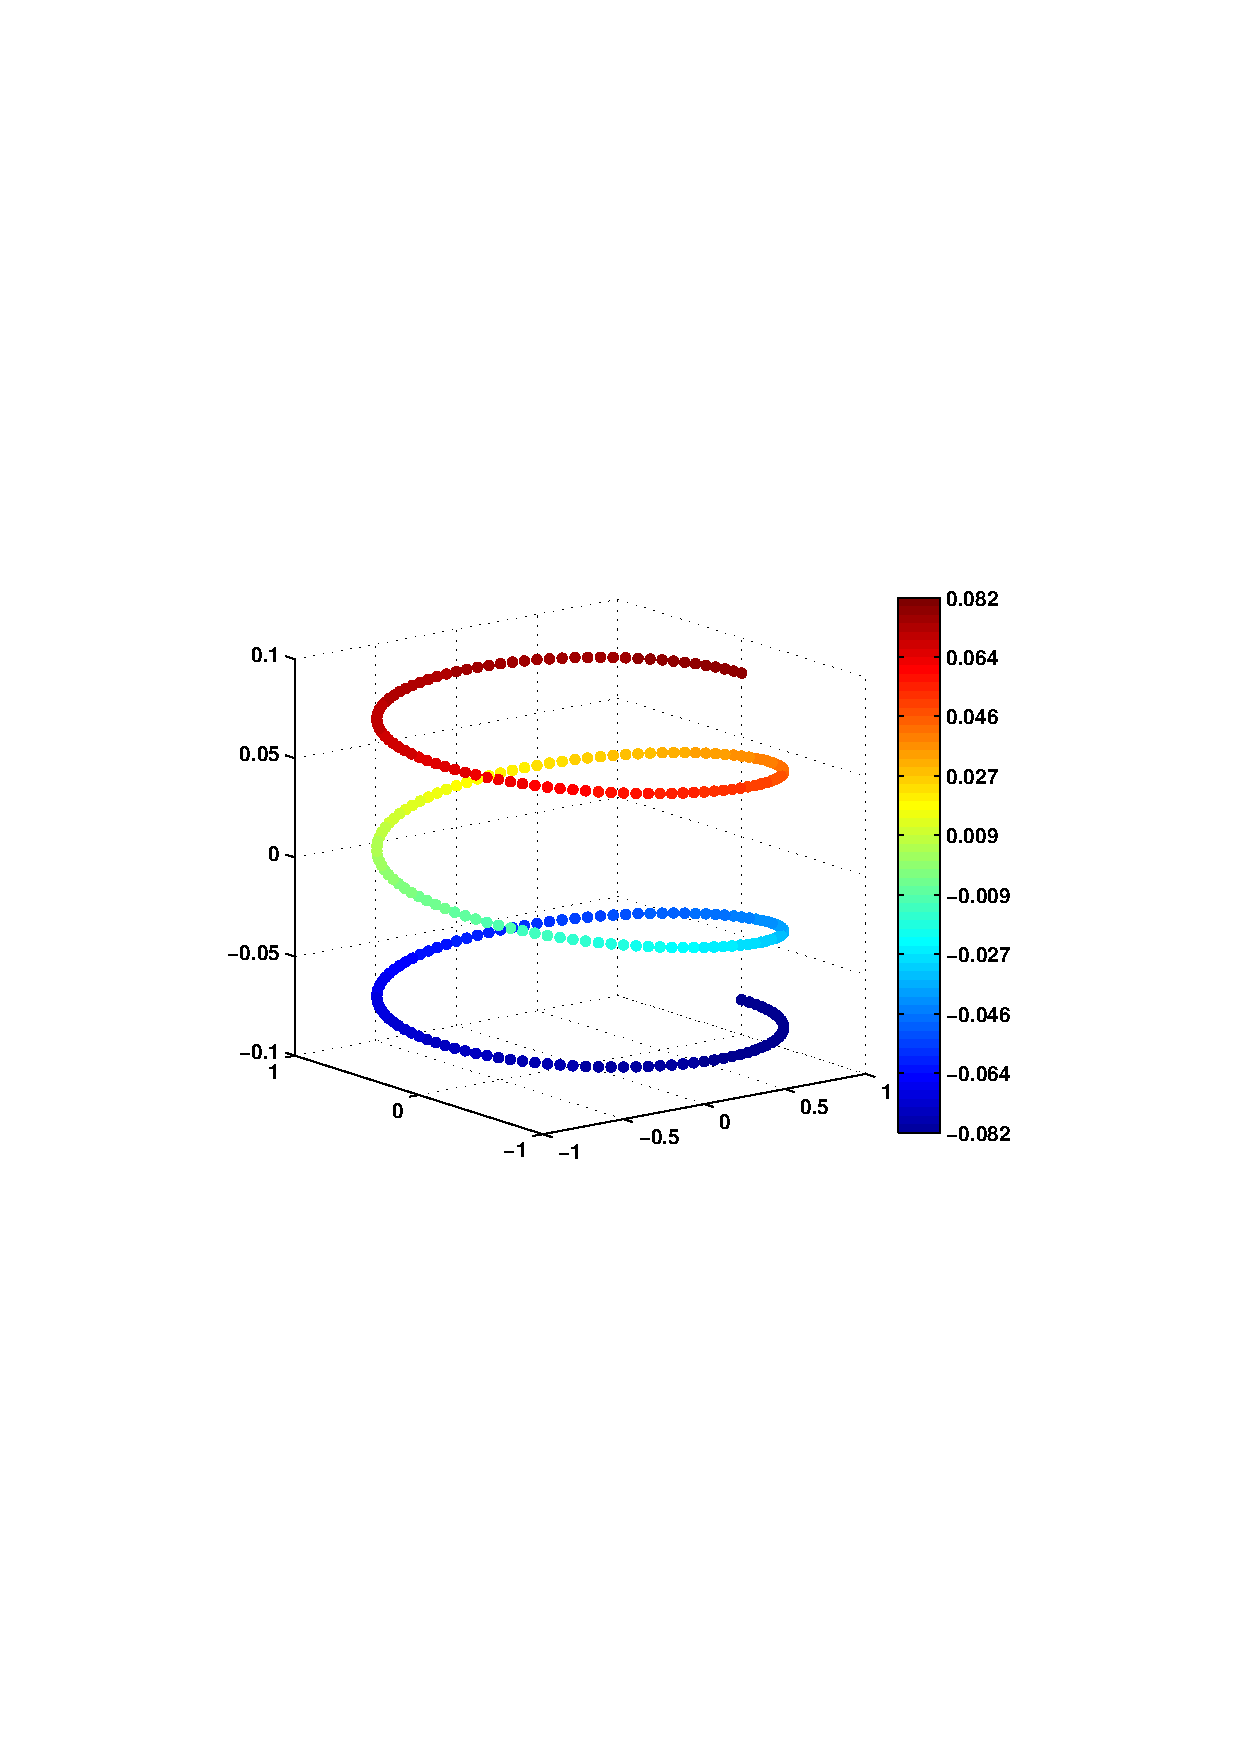
\includegraphics[width=0.45\textwidth]{helix.png}}
\end{figure}
\begin{itemize}
  \item Interesting results from Laplacian matrix.
  \item Develop new methods to obtain warm starting points.
\end{itemize}
}

\framee{Nonlinear Dimensionality Reduction}{
\begin{block}{Dimensionality Reduction Problem}
Given a set of $n$ points $x_1,\ldots, x_n$ in $\Real^l$, find a set of points $y_1,\ldots,y_n$ in $\Real^m (m\ll l)$ such that $y_i$ "represents" $x_i$.
\end{block}
Relation to DGP:\\
\begin{itemize}
  \item In noisy case, the distances can not be {\blue precisely} realized in low-dimensional space.
  \item If the distances in DGP do not contradict with each other, $n$ points can be {\blue precisely} realized in at most $n-1$ Euclidean space.
\end{itemize}

\begin{block}{Algorithm framework  ({\footnotesize Belkin-Niyogi, 2002})}
\begin{enumerate}[Step 1]
  \item Constructing the adjacency graph \\ (a) $\epsilon$-neighborhood \quad (b) $k$-nearest neighbors
  \item Choosing the weights \\ (a) Heat kernel \quad \quad ~~(b) Simple-minded
  \item Eigenmaps: $x_i\rightarrow (f_1(i),\ldots,f_m(i))$, where $Lf_i=\lambda_i Df_i$,\\ $0=\lambda_0 \leq \lambda_1 \leq \ldots \leq \lambda_{n-1}$.
\end{enumerate}
\end{block}
}

\framee{Laplacian Matrix}{
Given a graph $G=(V,E)$, the Laplacian matrix $L$ is defined by $L=D-W$, where
$$W_{ij} = \left \{
\begin{array}{ll}
e^{-\|x_i-x_j\|^2/t}  & if~ (i,j)\in E, \\
0                     & otherwise.
\end{array}
\right.$$
and $D$ is a diagonal matrix with
$$D_{ii}=\sum\nolimits_j W_{ij}.$$
Note that $W$ degenerate to the adjacent matrix when $t=\infty$.
}

\framee{Optimal Embedding}{
\begin{block}{}
Problem: Map the weighted graph $G$ to a line such that the adjacent vertices stay as close as possible.
\end{block}
Let $y=(y_1,y_2,\ldots,y_n)^T$ be such a map, we have
$$\frac{1}{2}\sum_{(i,j) \in E}(y_i-y_j)^2W_{ij}=y^TLy$$
Therefore,
$$\min_{y^TDy=1,Y^TDe=0} y^TLy$$
gives us a reasonable solution.
\pause
\vskip2mm
\begin{block}{}
General case: Embed the graph into $m$-dimensional Euclidean space.
\end{block}
Let $Y=[y_1 ~y_2~\ldots ~ y_n]^T\in \Real^{n\times m}$ that each row gives a coordinate. Similarity we need to minimize
$$\sum_{(i,j)\in E} \|y_i-y_j\|^2W_{ij} = tr(Y^TLY)$$.
}

\framee{Courant-Fischer Theorem}{
\begin{block}{Courant-Fischer Theorem}
Let $A$ be a symmetric $n\times n$ matrix with eigenvalues $\lambda_1 \leq \lambda_2 \leq \ldots \leq \lambda_n$ and corresponding eigenvectors $v_1,v_2,\ldots,v_n$. For $1\leq k \leq n$, let $S_k$ denote the span of $v_1,\ldots,v_k$ (with $S_0=\{0\}$), and let $S_k^{\bot}$ denote the orthogonal complement of $S_k$. Then
$$\lambda_k = \min_{\|x\|=1,x\in S_{k-1}^{\bot}} x^TAx = \min_{x\in S_{k-1}^{\bot}} \frac{x^TAx}{x^Tx}$$
\end{block}
}

\framee{Toy Example 1}{
\begin{figure}
  \centering
  \includegraphics[width=0.85\textwidth]{1.jpg}\\
  \caption{cutoff=2, degree: [4,2,3.4], noise = 20\%}
\end{figure}
}

\framee{Toy Example 1}{
\begin{figure}
  \centering
  \includegraphics[width=0.85\textwidth]{2.jpg}\\
  \caption{cutoff=4, degree: [8,4,6], noise = 20\% }
\end{figure}
}

\framee{Random Example 1}{
\begin{figure}
  \centering
  \includegraphics[width=0.85\textwidth]{3.jpg}\\
\end{figure}
}

\framee{Random Example 2}{
\begin{figure}
  \centering
  \includegraphics[width=0.85\textwidth]{4.jpg}\\
\end{figure}
}

\framee{Toy Example 2}{
\begin{figure}
  \centering
  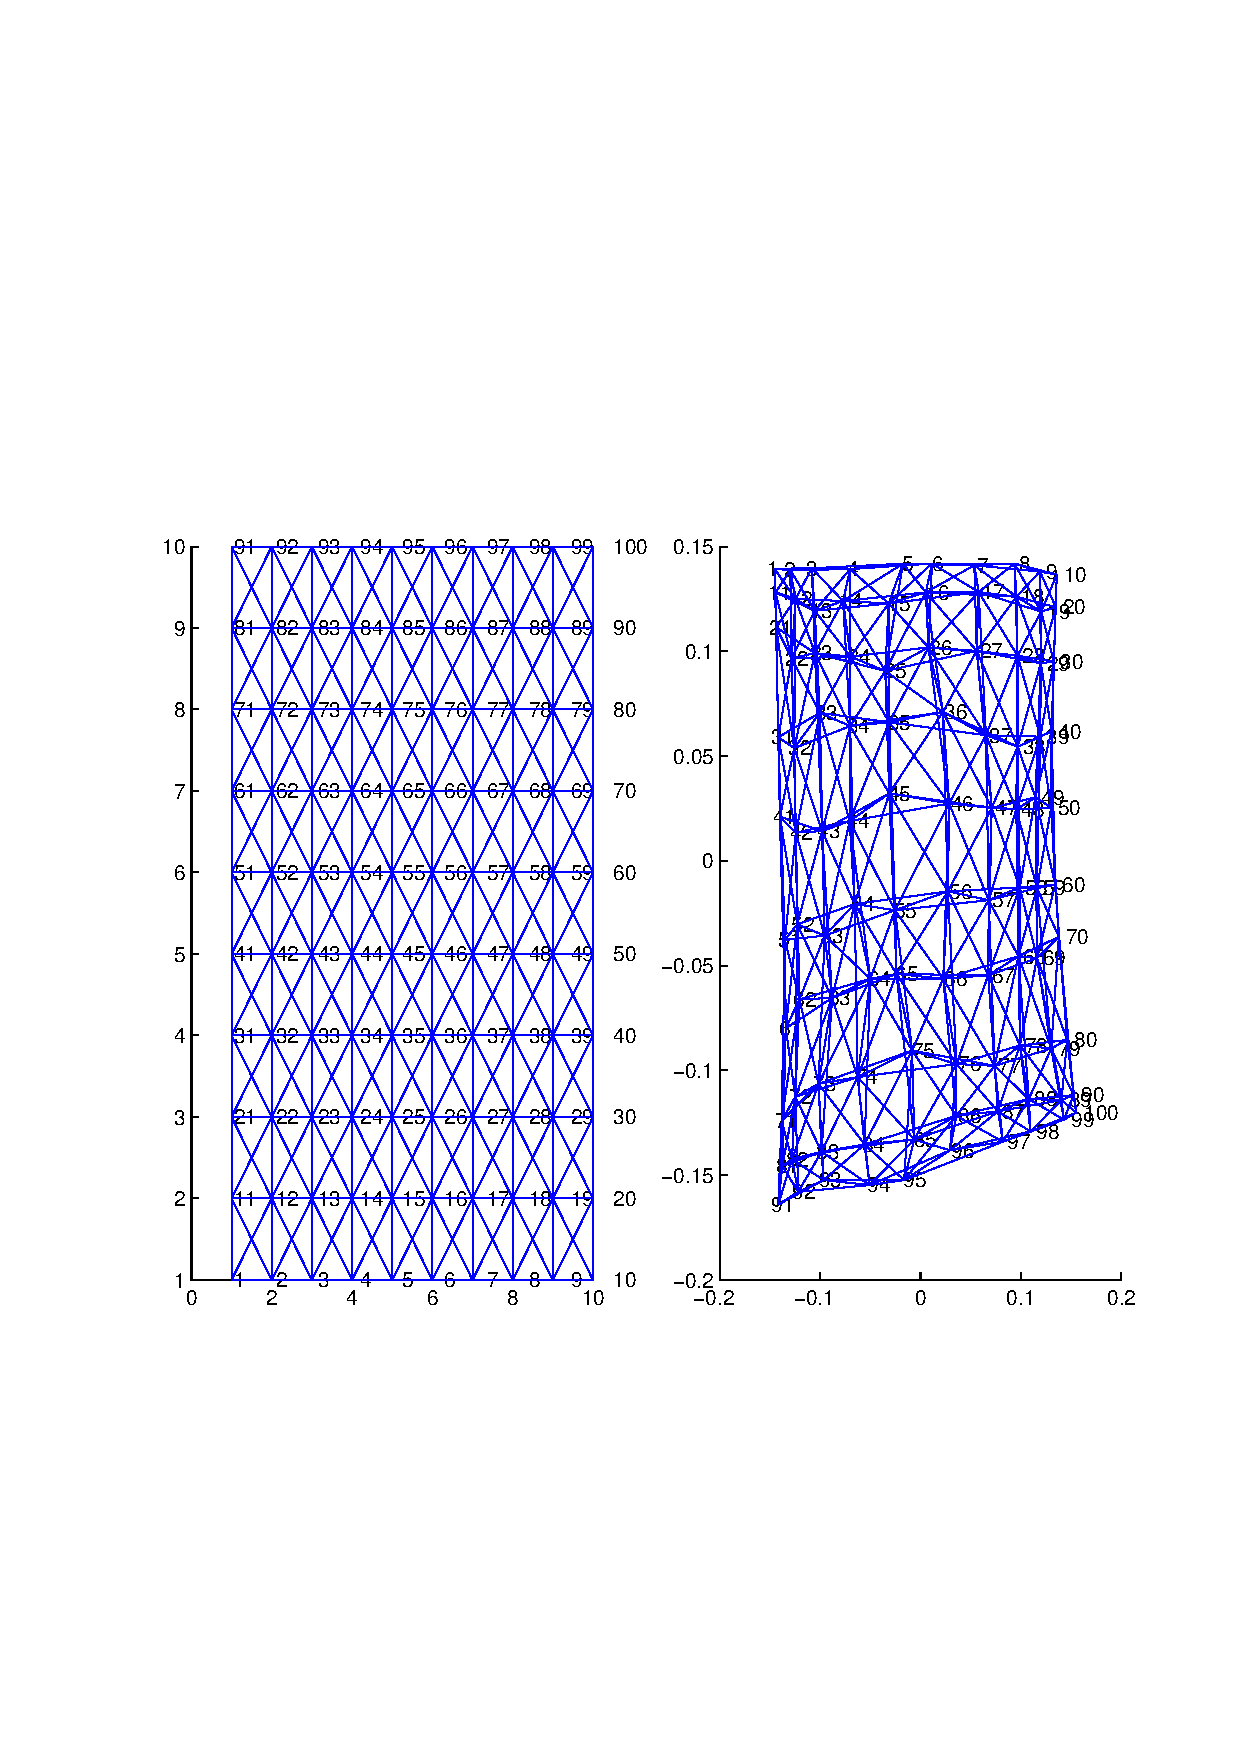
\includegraphics[width=0.85\textwidth]{5.jpg}\\
  \caption{cutoff=2, degree: [12,5,10], noise = 20\%}
\end{figure}
}

\framee{Toy Example 2}{
\begin{figure}
  \centering
  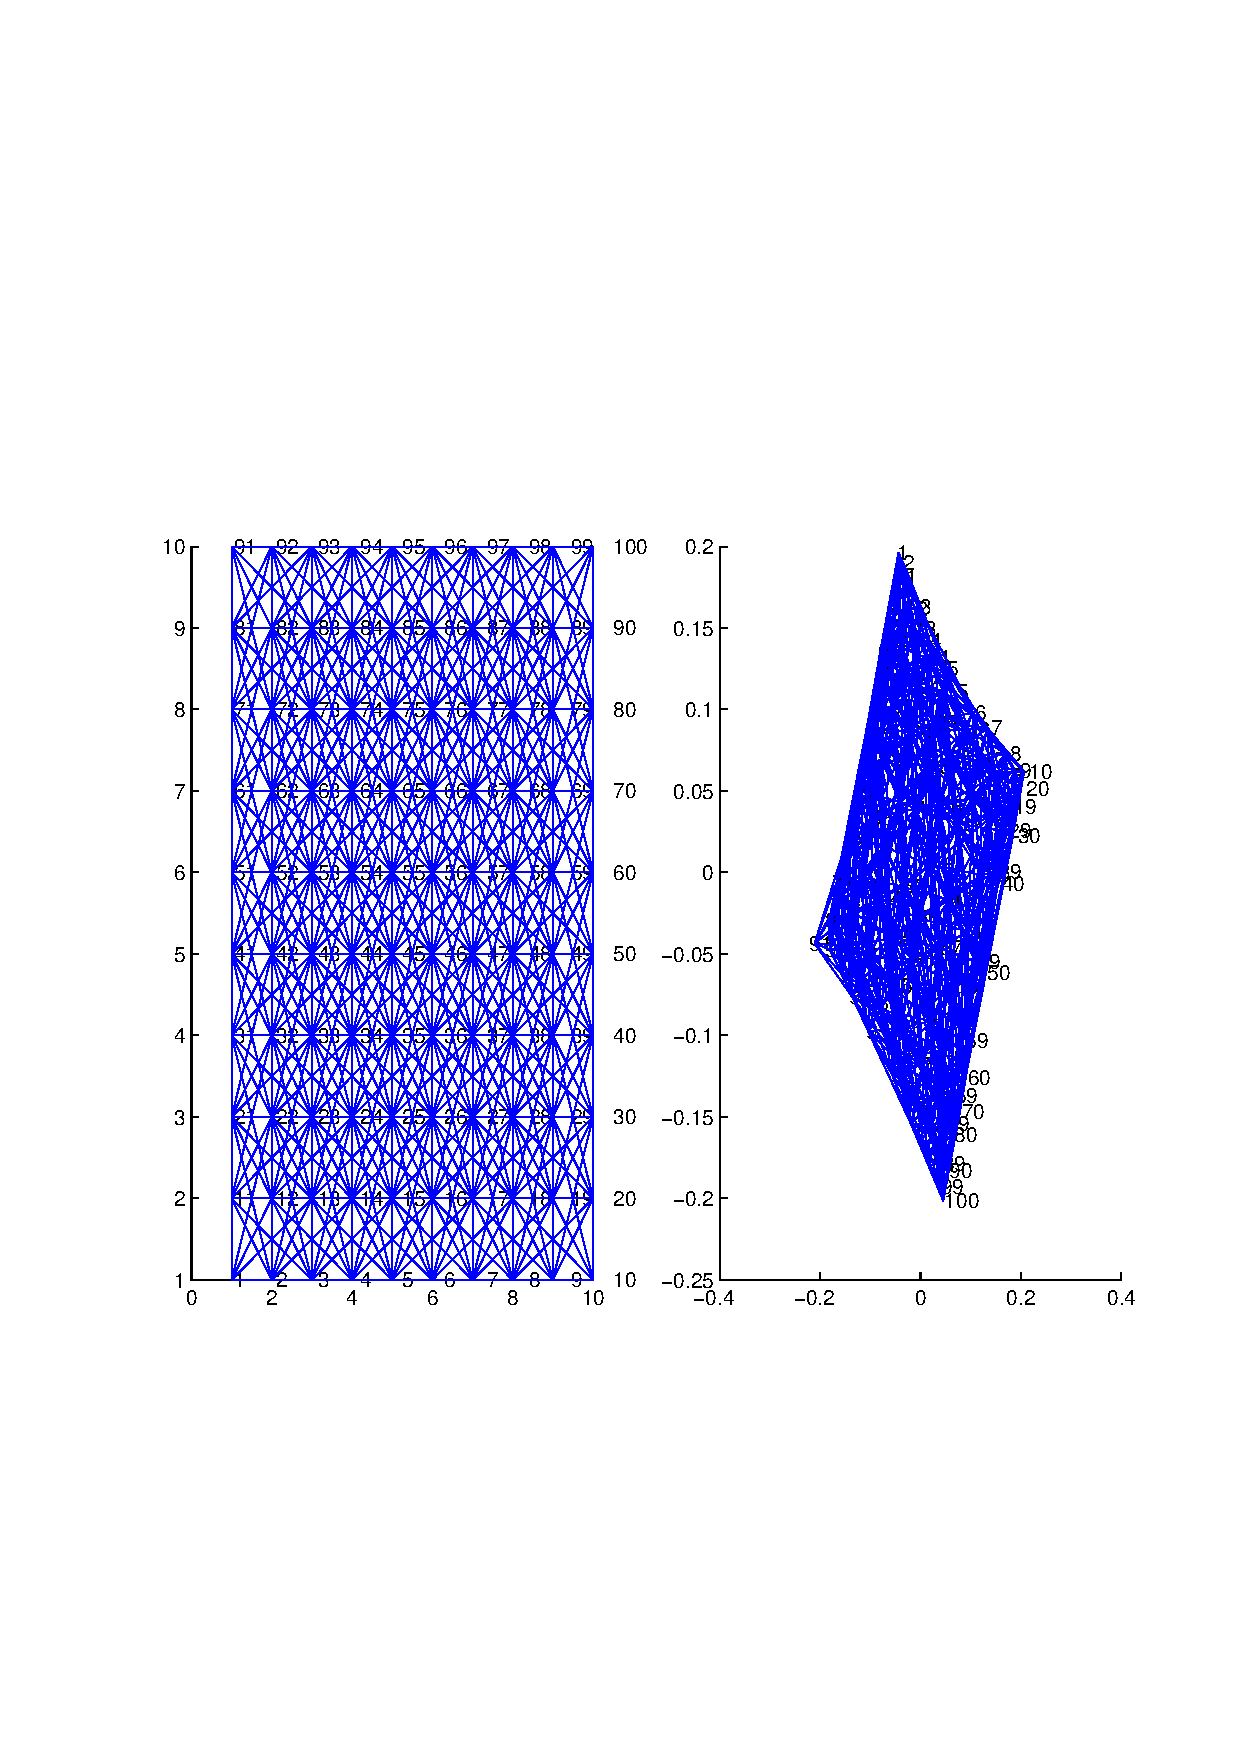
\includegraphics[width=0.85\textwidth]{6.jpg}\\
  \caption{cutoff=3, degree: [20,10,21.2], noise = 20\%}
\end{figure}
}

\framee{Random Example 3}{
\begin{figure}
  \centering
  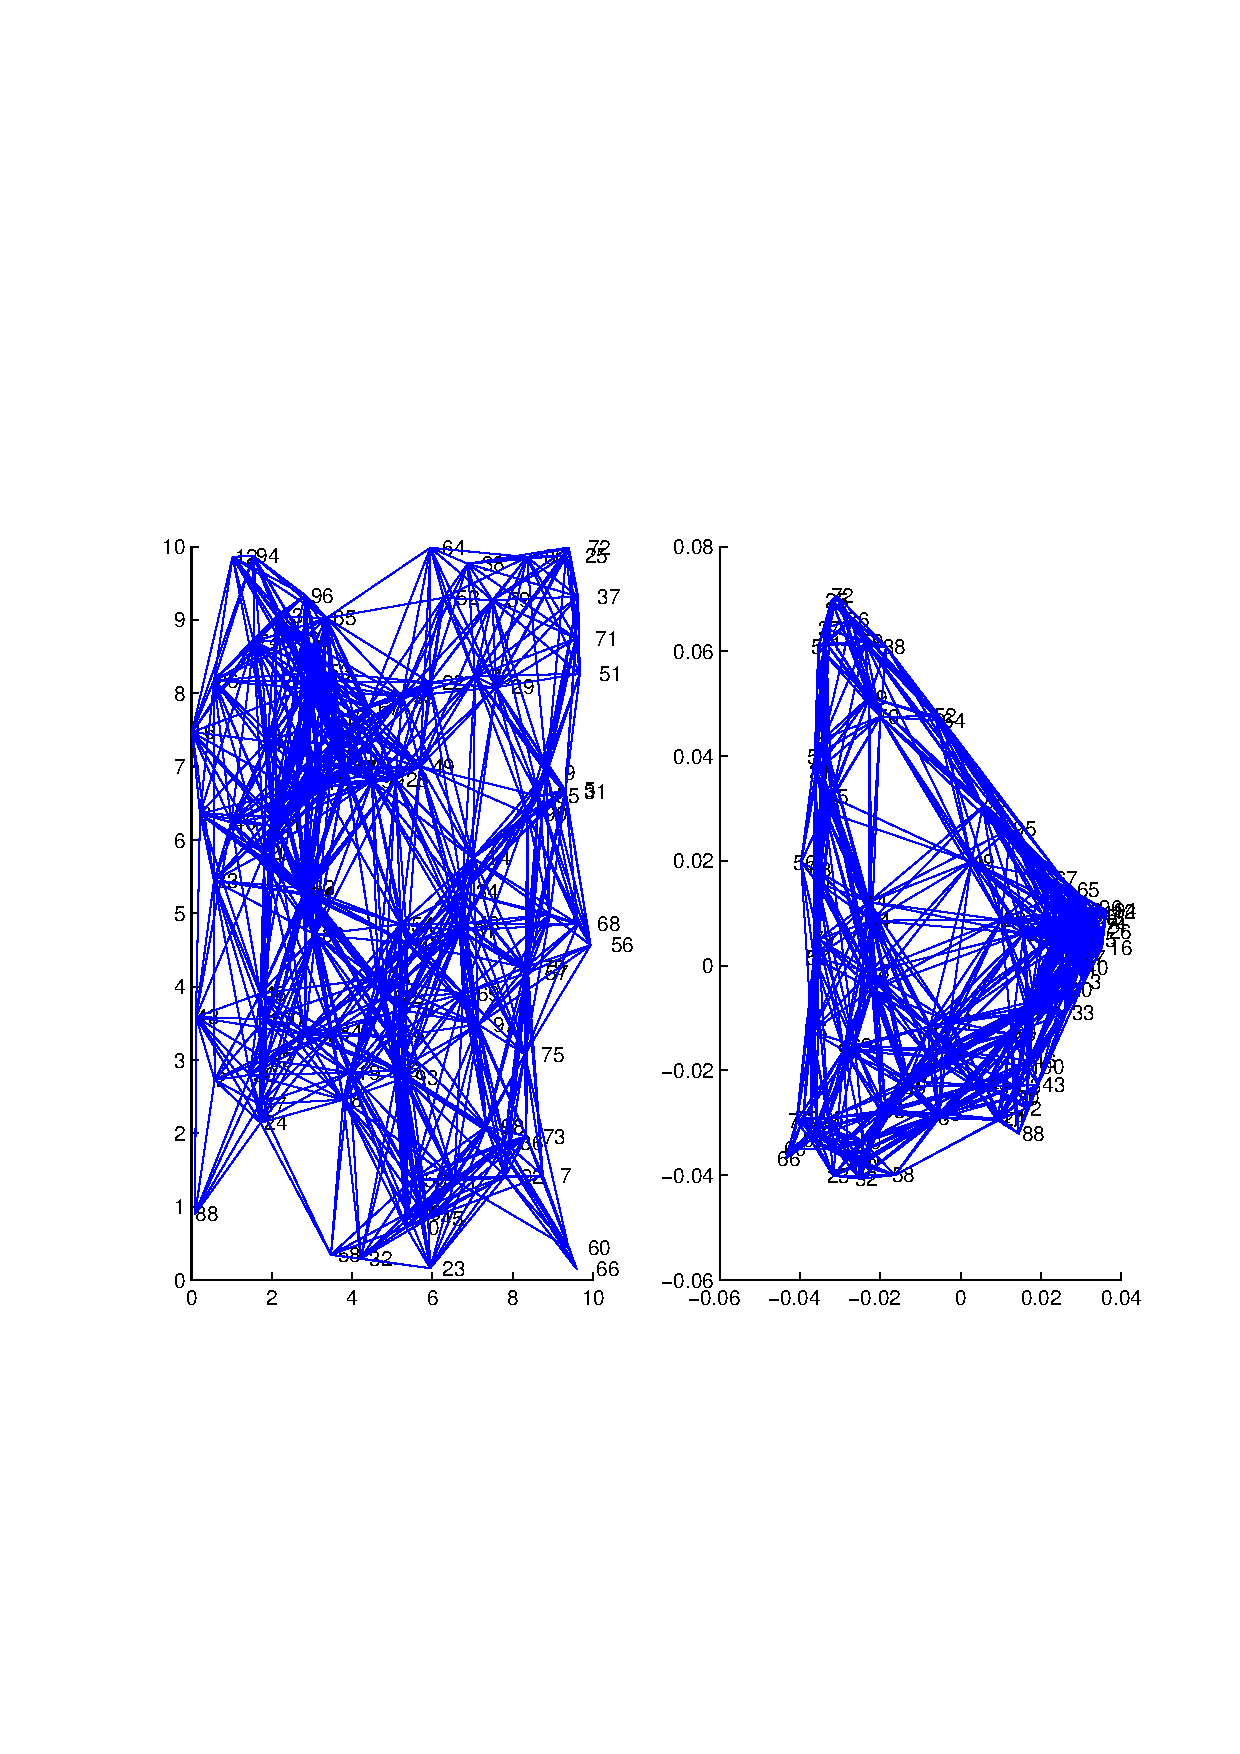
\includegraphics[width=0.85\textwidth]{7.jpg}\\
\end{figure}
}

\framee{Random Example 4}{
\begin{figure}
  \centering
  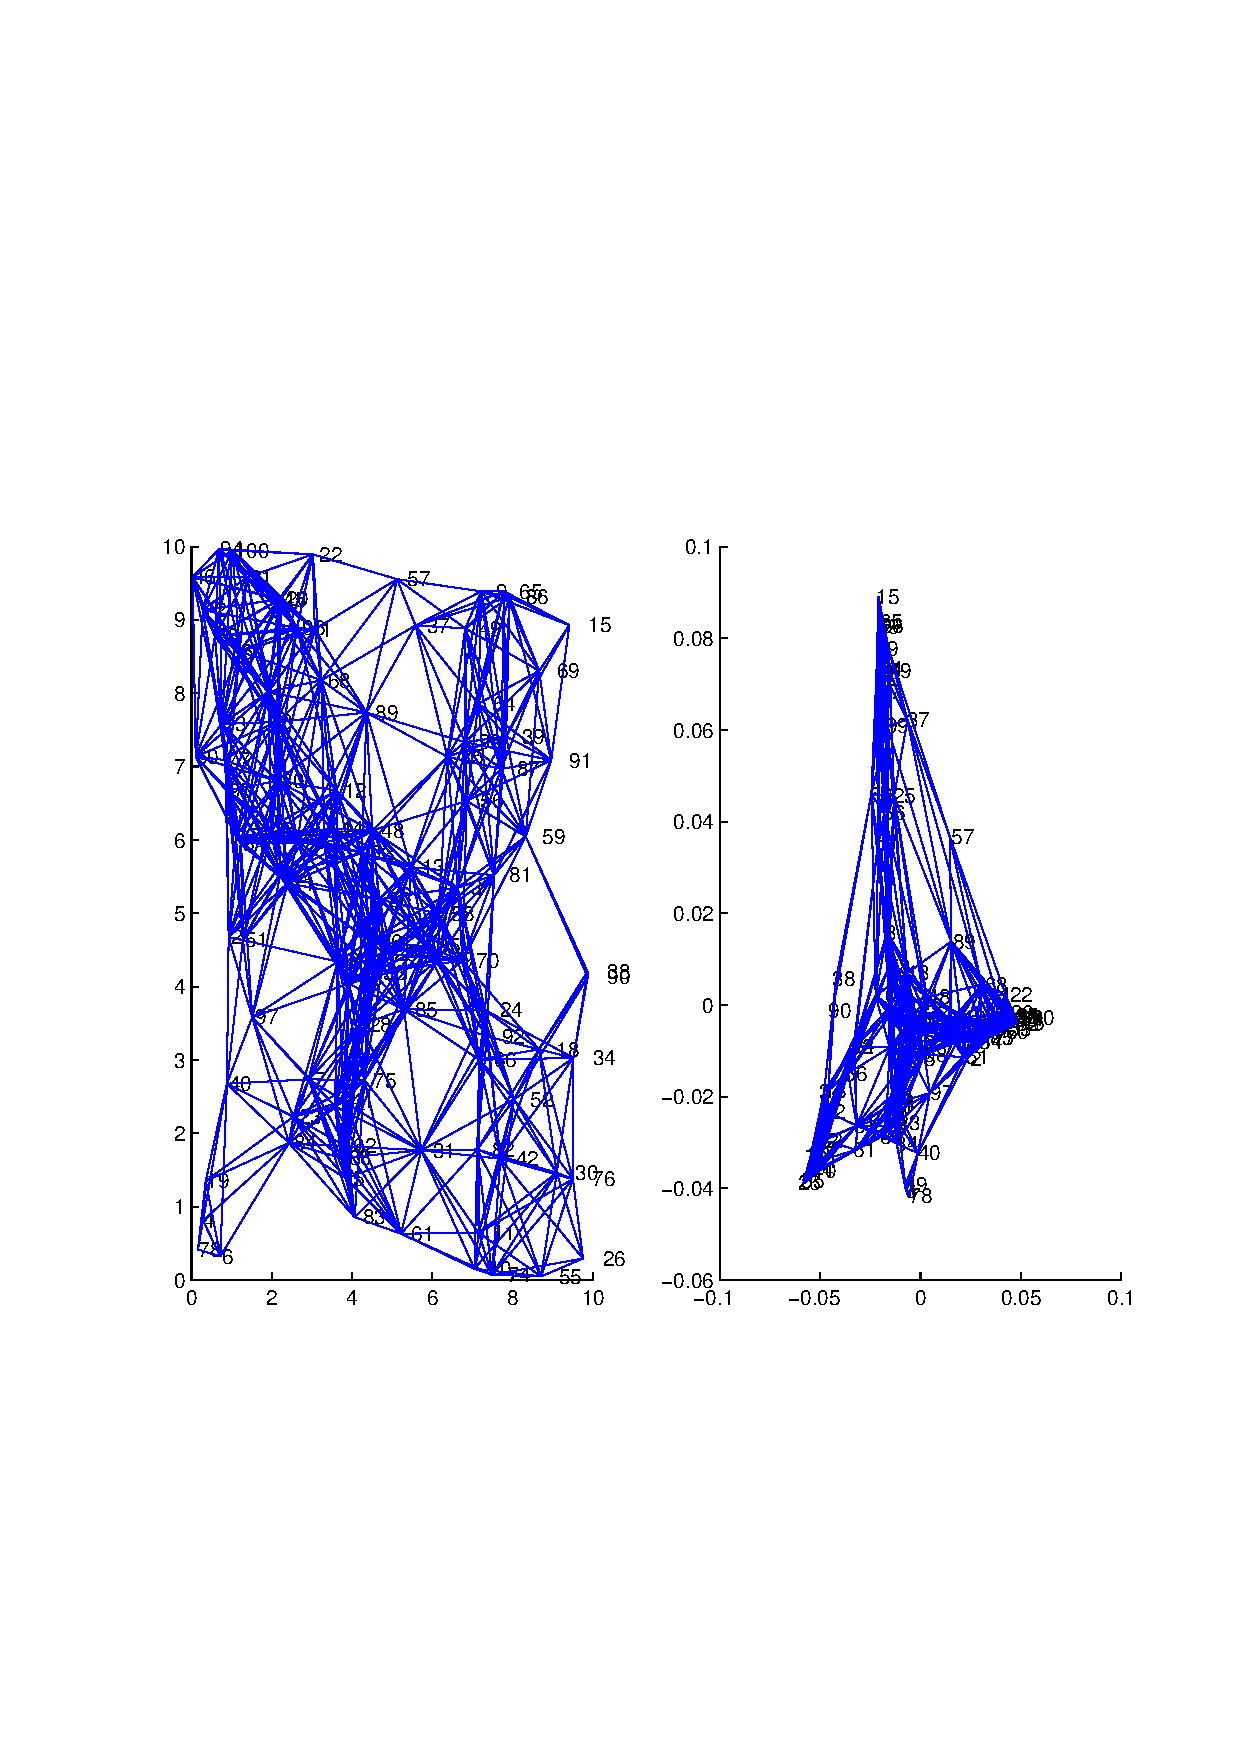
\includegraphics[width=0.85\textwidth]{8.jpg}\\
\end{figure}
}


\framee{}{
Observations:
\begin{itemize}
  \item With or without $D$, they make no big difference.
  \item The results vary slightly as $\epsilon /k, t$ change.
  \item The result is {\blue reasonably robust} w.r.t the noise in distances.
  \item It performs better in "uniform" graphs.
  \item Sometimes several points collapse to stay together, which is due to the way we construct distances.
  \item It does not give the right coordinates, but meaningful topology information.
\end{itemize}
}

\subsection{Algorithm Framework}
\framee{Algorithm framework}{
\begin{block}{Laplacian Eigenmap-based Algorithm for DGP}
\begin{enumerate}[Step 1]
  \item Construct the Laplacian matrix $L$ and calculate its eigenvalue decomposition $L=VDV^T$ such that the eigenvalues in $D$ are in ascending order.
  \item Set $X0 = V(:,2:m+1)$ and scale it to the proper magnitude.
  \item Using $X0$ as the initial point, apply error function minimization method to further improve the result.
\end{enumerate}
\end{block}
}

\framee{Scale}{
Note that the coordinates from Eigenvalue decomposition only reveals the topology, but not in the right magnitude, therefore scaling the points is necessary.
\begin{enumerate}
  \item Construct a new distance matrix $\tilde{D}$ according to $X0$ and $E$.
  \item Calculate
      $$ratio = \frac{sum(D)}{sum(\tilde{D})}.$$
  \item Set $X0 = X0*ratio$.
\end{enumerate}
}

\subsection{Numerical Experiments}
\framee{Toy Example 2}{
\begin{figure}
  \centering
  \subfigure{\includegraphics[width=0.4\textwidth]{9.jpg}}
  \subfigure{\includegraphics[width=0.4\textwidth]{10.jpg}}
  \subfigure{\includegraphics[width=0.4\textwidth]{11.jpg}}
  \subfigure{\includegraphics[width=0.4\textwidth]{12.jpg}}
  \caption{cutoff = 2, noise = 0, 5\%, 10\%, 20\%}
\end{figure}
}

\framee{Random Example}{
\begin{figure}
  \centering
  \includegraphics[width=0.8\textwidth]{13.jpg}\\
  \caption{cutoff = 3, noise = 0}
\end{figure}
}

\framee{Random Example}{
\begin{figure}
  \centering
  \includegraphics[width=0.8\textwidth]{14.jpg}\\
  \caption{cutoff = 3, noise = 5\%}
\end{figure}
}

\framee{Random Example}{
\begin{figure}
  \centering
  \includegraphics[width=0.8\textwidth]{15.jpg}\\
  \caption{cutoff = 3, noise = 10\%}
\end{figure}
}

\framee{}{
\begin{figure}
  \centering
  \includegraphics[width=0.85\textwidth]{1PTQ50.jpg}\\
  \caption{1PTQ:402, cutoff = 5, noise = 0}
\end{figure}
}

\framee{}{
\begin{figure}
  \centering
  \includegraphics[width=0.85\textwidth]{1PTQ60.jpg}\\
  \caption{1PTQ:402, cutoff = 6, noise = 0}
\end{figure}
}

\framee{}{
\begin{figure}
  \centering
  \includegraphics[width=0.85\textwidth]{1PTQ65.jpg}\\
  \caption{1PTQ:402, cutoff = 6, noise = 5\%}
\end{figure}
}


\section{Conclusion and Future Work}
\frame{
\frametitle{Conclusion and Future Work}
\begin{itemize}
\item Conclusion
    \begin{itemize}
        \item Proposed a Laplacian Eigenmap-based algorithm for DGP.
        \item Finished some very preliminary numerical experiments.
    \end{itemize}
\item Future Work
    \begin{itemize}
      \item Figure out the problem with protein computation.
      \item Carefully study the parameters in Laplacian matrix.
      \item Eliminate some edges to reduce the computational complexity in nonlinear programming.
      \item Develop new error functions to model the problem better.
      \item Try to develop distributed algorithm based Laplacian Eigenmap.
    \end{itemize}
\end{itemize}
}


\frame{
%\frametitle{Q \& A}
\begin{center}
  \Large{  \textsc{Thank you for your attention!}}  \\
  \vspace{0.2cm}
  {\blue szl@lsec.cc.ac.cn }
\end{center}
}

\end{CJK*}
\end{document}
